\chapter{Event Reconstruction}

In this chapter the procedure for event reconstruction of the $B$ meson decay $B \to K K \ell \nu$ is shown, starting with final state particle selection and then combining them to obtain $B$ meson candidates.

\section{Final State Particles Selection}
Since the neutrino escapes detection, we can only reconstruct the charged tracks in the decay, which are the two charged kaons ($K$) and the light lepton, which is the electron ($e$) or muon ($\mu$). These are some of the particles which are commonly referred to as final state particles (FSP). Final state particles have a long lifetime and are usually the particles that we detect when they interact with the material in the detector.

It is important to limit our selection of FSP particles in order to cut down the number of particle combinations, and consequentially computation time and file sizes.

At this point in the analysis, we do not apply any intelligent cuts yet, which results in a large number of available particles and their combinations. In order to minimize this effect, we perform this part of the study on a smaller subset of the available generic MC, experiment no. $23$ and $31$, which correspond to an integrated luminosity of $6.273\e{fb^{-1}}$ and $17.725\e{fb^{-1}}$, respectively. We chose these two experiments to get closer to the appropriate ratio of SVD1 and SVD2 data in the full Belle MC.

\subsubsection{Leptons}

Figures \ref{fig:evars} and \ref{fig:muvars} show the impact parameters $d_0$ and $z_0$, the momentum in  $\Upsilon(4S)$ center-of-mass system (CMS), and the PID information for true and fake electrons and muons, where an extra category for true electrons/muons from the signal decay is shown.

\begin{figure}[H]
	\centering
	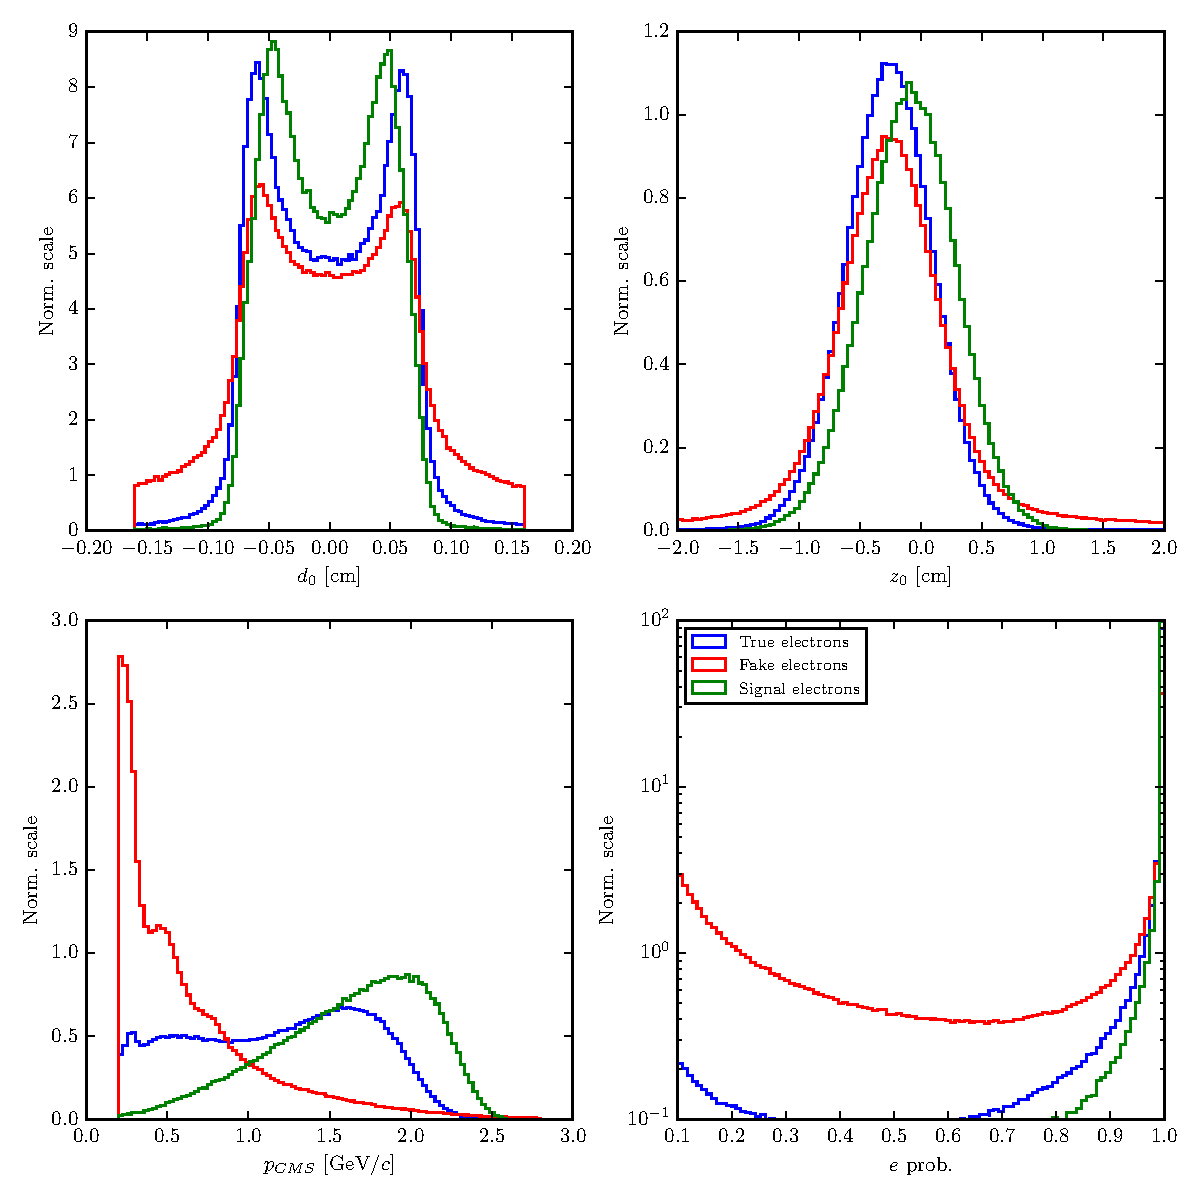
\includegraphics[width=\linewidth]{fig/FSP_e_vars}
	\captionsetup{width=.8\linewidth}
	\caption{Normalized properties of true (blue), fake (red) and true electrons from signal $B$ candidates (green).}
	\label{fig:evars}
\end{figure}

\begin{figure}[H]
	\centering
	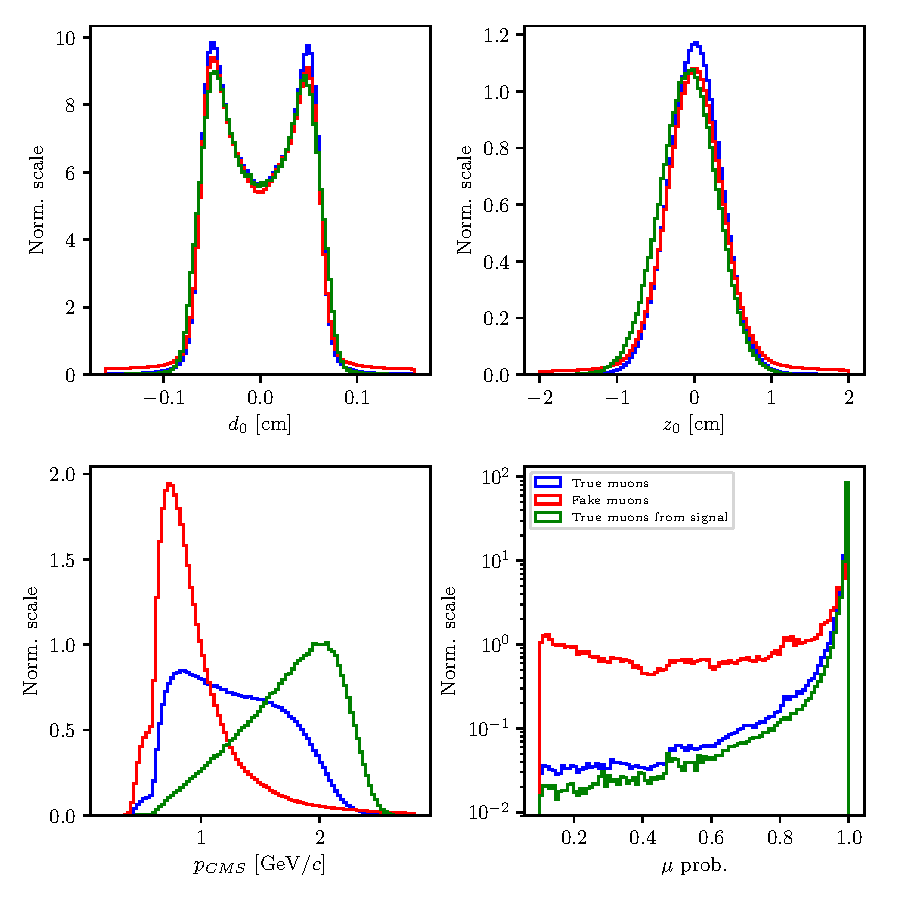
\includegraphics[width=\linewidth]{fig/FSP_mu_vars}
	\captionsetup{width=.8\linewidth}
	\caption{Normalized properties of true (blue), fake (red) and true muons from signal $B$ candidates (green).}
	\label{fig:muvars}
\end{figure}

Based on these distributions, we can define a set of cuts
\begin{itemize}
	\item $\vert d_0 \vert < 0.1\e{cm}$,
	\item $\vert z_0 \vert < 1.5\e{cm}$,
	\item $p_{CMS} \in [0.4,\,2.6]~\e{GeV}/c$ for electrons,
	\item $p_{CMS} \in [0.6,\,2.6]~\e{GeV}/c$ for muons.
\end{itemize}

After this selection we can determine the optimal PID cuts for electrons and muons, where we optimize the selection by maximizing the standard definition of \textit{figure of merit} ($\mathrm{FOM}$), defined in Eq. (\ref{eq:fom})
\begin{equation}
\label{eq:fom}
\mathrm{FOM} = \sqrt{\mathcal{E}\mathcal{P}} \propto \frac{S}{\sqrt{S+B}},
\end{equation} 
where the argument in the square root is the product of the efficiency ($\mathcal{E}$) and the purity ($\mathcal{P}$) function. The definitions of signal ($S$) and background ($B$) are somewhat fluid throughout the analysis and need to be defined for each $\mathrm{FOM}$ separately. In this section we define two representations of $S$ and $B$. In $\mathrm{FOM}_1$ the signal $S$ represents correctly reconstructed final state particles, while in $\mathrm{FOM}_2$ the signal $S$ represents correctly reconstructed final state particles which also come from a correctly reconstructed $B$ meson candidate. In both cases $B$ represents all other particle candidates which do not satisfy the conditions of $S$.

The $\mathrm{FOM}$ plots are shown in Figures \ref{fig:efom} and \ref{fig:mufom}. The cut values are based on PID cuts used for PID efficiency calibration. The optimal value for the PID cuts is equal to the largest available value, regardless of the leptons coming from signal decays or not. The optimized PID cuts for leptons are
\begin{itemize}
	\item $e$ prob. $ > 0.9$ for electrons,
	\item $\mu$ prob. $ > 0.97$ for muons.
\end{itemize}

\begin{figure}[H]
	\centering
	\captionsetup{width=.8\linewidth}
	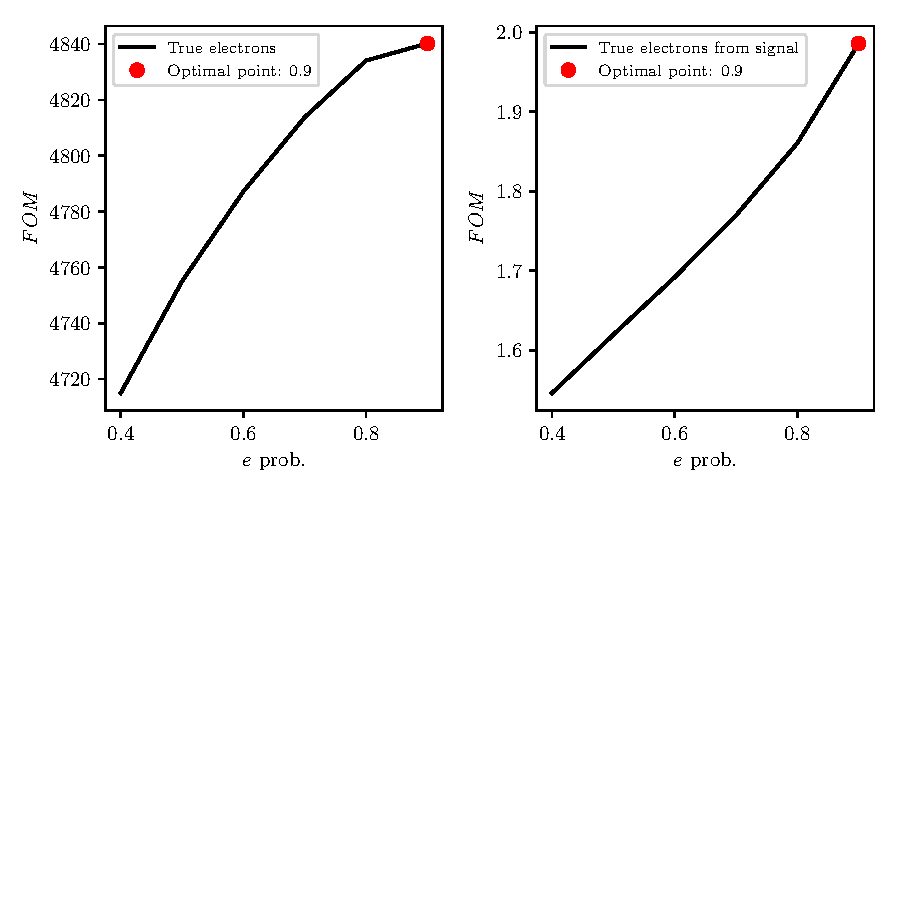
\includegraphics[width=\linewidth]{fig/FSP_e_fom}
	\caption{$\mathrm{FOM}$ optimizations of the PID probability cuts for true electrons (left) and true electrons from signal $B$ candidatess (right).}
	\label{fig:efom}
\end{figure}

\begin{figure}[H]
	\centering
	\captionsetup{width=.8\linewidth}
	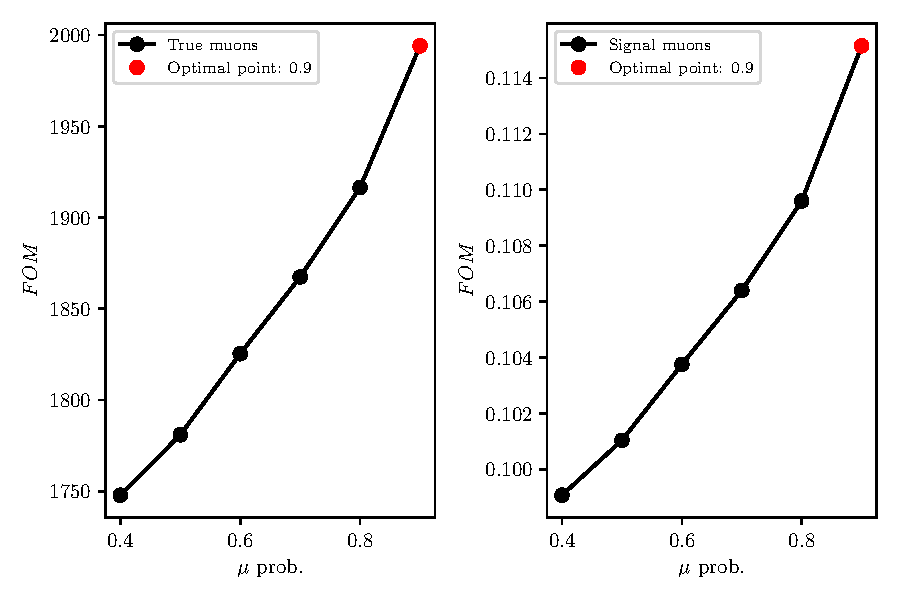
\includegraphics[width=\linewidth]{fig/FSP_mu_fom}
	\caption{$\mathrm{FOM}$ optimizations of the PID probability cuts for true muons (left) and true muons from signal $B$ candidates (right).}
	\label{fig:mufom}
\end{figure}


\subsubsection{Kaons}

We repeat the procedure for both kaons. Figure \ref{fig:Kvars} shows the impact parameters $d_0$ and $z_0$, the momentum in  $\Upsilon(4S)$ center-of-mass system (CMS), and the PID information for true and fake kaons, where an extra category for true kaons from the signal decay is shown.

\begin{figure}[H]
	\centering
	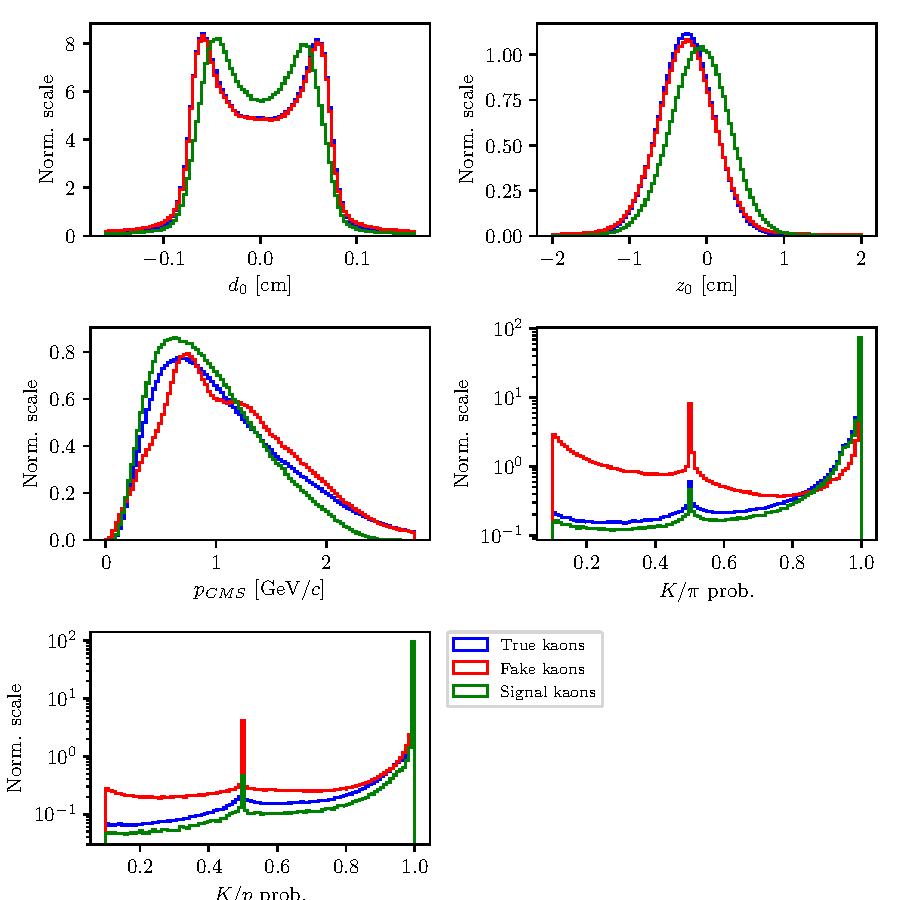
\includegraphics[width=\linewidth]{fig/FSP_kaon_vars}
	\captionsetup{width=.8\linewidth}
	\caption{Normalized properties of true (blue), fake (red) and true kaons (green) from signal $B$ candidates.}
	\label{fig:Kvars}
\end{figure}

We define the kaon cuts in the same manner as in the case for leptons
\begin{itemize}
	\item $\vert d_0 \vert < 0.15\e{cm}$,
	\item $\vert z_0 \vert < 1.5\e{cm}$,
	\item $p_{CMS} \in [0,\,2.5]~\e{GeV}/c$.
\end{itemize}

The PID optimization, in this case, is taken in two steps. First, we optimize the cut on $K / \pi$, and after that the $K/p$ separation probability. Figure \ref{fig:Kfom} shows the optimization procedure for PID cuts on kaon candidates.

\begin{figure}[H]
	\centering
	\captionsetup{width=.8\linewidth}
	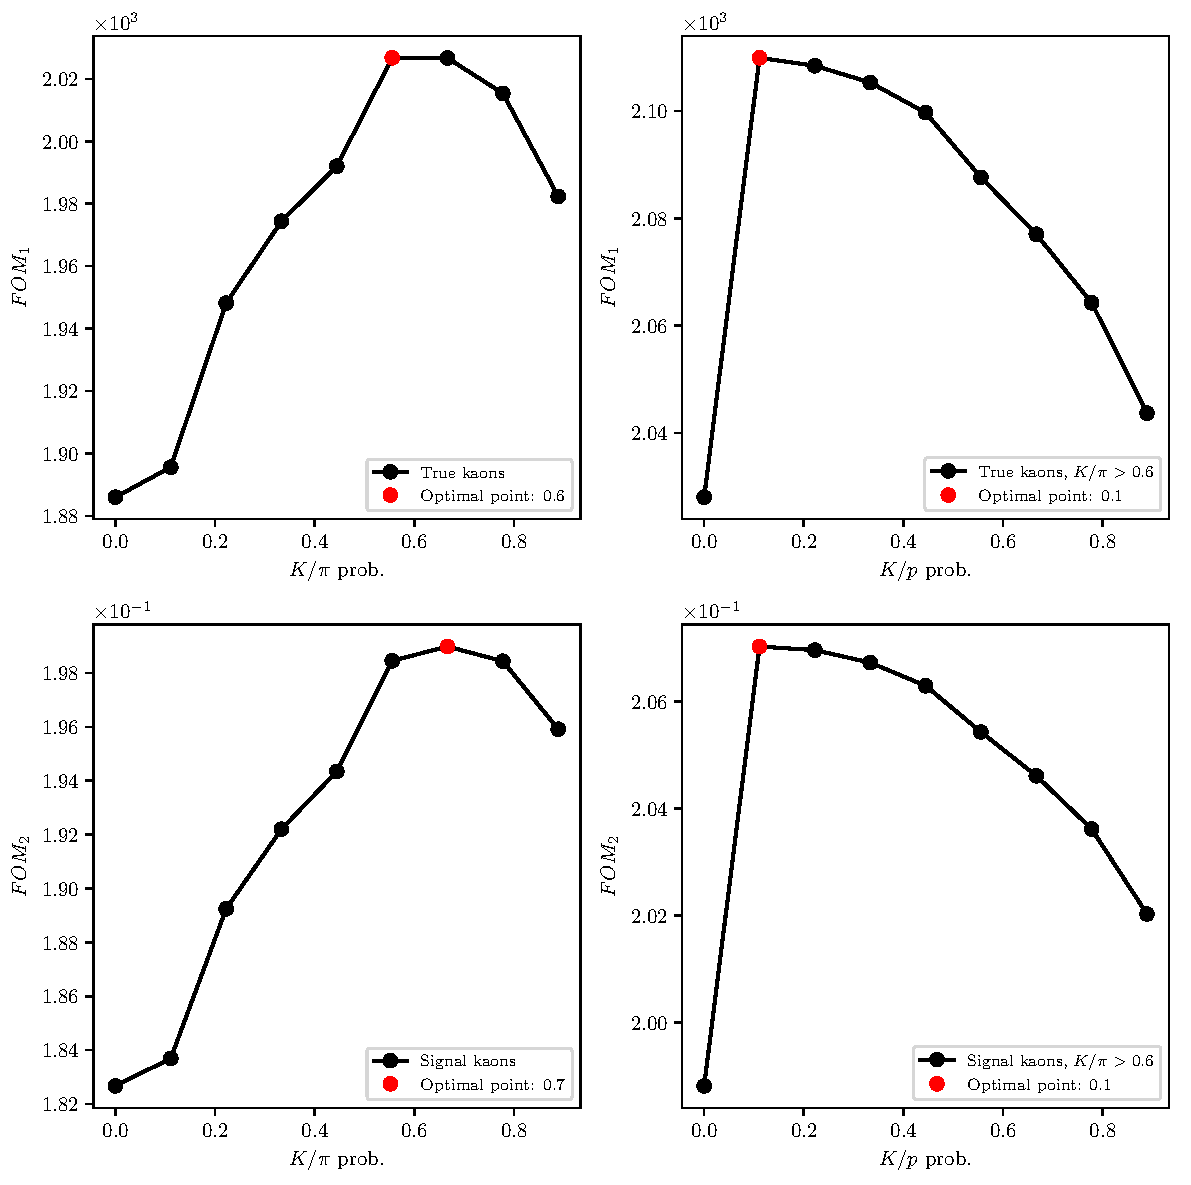
\includegraphics[width=\linewidth]{fig/FSP_kaon_fom}
	\caption{$\mathrm{FOM}$ optimizations of the PID probability cuts for true kaons (top) and true kaons from signal $B$ candidates (bottom). The plots on the left show the optimization of the first step for the $K / \pi$ probability cut, and the plot on the right the $K/p$ probability cut.}
	\label{fig:Kfom}
\end{figure}

The optimized PID cuts for kaons are
\begin{itemize}
	\item $K/\pi > 0.6$,
	\item $K/p > 0.1$.
\end{itemize}

\section{Pre-selection of First $B$ Meson Candidates}

In this section, we use the charged particle candidates from the previous section to make particle combinations, which correspond to $B$ meson candidates. When a $B$ meson candidate is selected, additional features can be calculated and used for background rejection. Since we are still performing this part of the study on a smaller subset of the full available MC sample, we will perform under-optimized cuts based on the FOM optimization in order to optimize them later on the full Belle MC sample.

Since the missing neutrino escapes detection, we reconstruct the $B$ mesons in the following two channels
\begin{align*}
B^+ &\to K^+ K^- e^+, \\
B^+ &\to K^+ K^- \mu^+,
\end{align*}
and similarly for $B^-$. When an arbitrary combination is obtained, we perform a vertex fit of the three tracks in order to discard combinations with a low probability of tracks coming from the same point. $B$ mesons have a relatively long lifetime and decay along the $z$ axis of the detector in the direction of the boost, so the vertex fit is enforced with an \texttt{IPTUBE} constraint, which constrains the vertex to an elongated ellipsoid along beam direction. We demand that the fit converged and apply a cut on the minimal fit probability. The fit probability for signal and background $B$ meson candidates is shown in Figure \ref{fig:vtx} (left). We perform a $\mathrm{FOM}$ cut optimization of this variable, which is shown in Figure \ref{fig:vtx} (right) for the subset of the Belle MC sample. In this and in the following cases, the definition of $S$ from Eq. (\ref{eq:fom}) are correctly reconstructed $B$ meson candidates with a missing neutrino which are not coming from a $b \to c$ transition.

\begin{figure}[H]
	\centering
	\captionsetup{width=0.8\linewidth}
	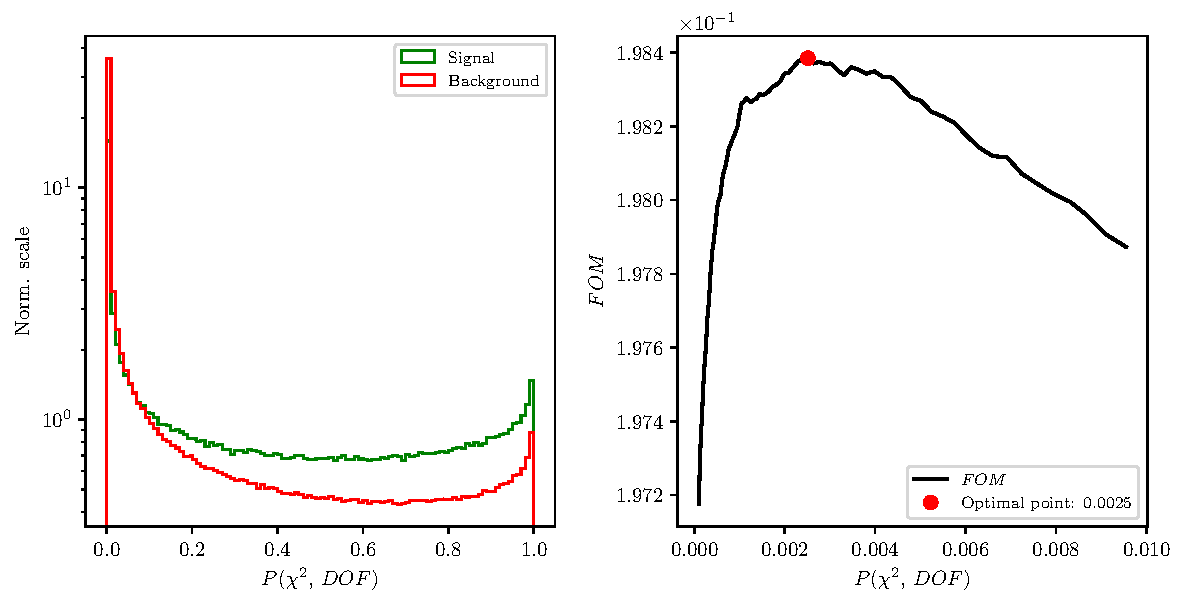
\includegraphics[width=\linewidth]{fig/VTX}
	%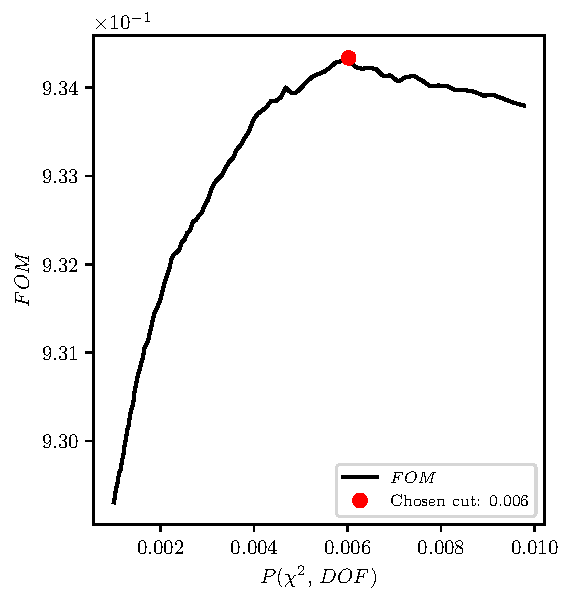
\includegraphics[width=\linewidth]{fig/VTX_precise}
	\caption{Normalized vertex fit probability distribution for signal and background $B$ meson candidates in logarithmic scale(left) and $\mathrm{FOM}$ optimization of the vertex fit probability (right) for the subset of the full Belle MC sample.}
	\label{fig:vtx}
\end{figure}

The chosen pre-cut on the fit probability is
\begin{itemize}
	\item $P(\chi^2,NDF) > 1.0\E{-3}$.
	%\item Optimal cut: $P(\chi^2,NDF) > 6.0\E{-3}$.
\end{itemize}

With the neutrino being the only missing particle on the reconstructed side, it is possible to determine the angle between the direction of the reconstructed $B$ (denoted as $Y \to K K \ell$) and the nominal $B$, as

\begin{align}
\mathrm{p}_\nu &= \mathrm{p}_B - \mathrm{p}_{Y}, \\
\label{eq:massnu}
\mathrm{p}_\nu^2 = m_\nu^2 &= m_B^2 + m_Y^2 - 2E_BE_Y + 2\vec{p}_B \cdot \vec{p}_Y \approx 0, \\ 
\label{eq:cosby}
\cos \left(\theta_{BY}\right) &= \frac{2E_BE_Y - m_B^2 - m_Y^2}{2\vert \vec{p}_B \vert \vert \vec{p}_Y\vert},
\end{align} 

where all the energy and momenta above are calculated in the CMS frame. The mass of the neutrino is equal to 0 to a very good precision, so we use it in Eq. (\ref{eq:massnu}). In addition, we can substitute the unknown energy and momentum magnitude, $E_B$ and $\vert \vec{p}_B \vert$, of the $B$ meson in Eq. (\ref{eq:cosby}), with quantities from the well known initial conditions
\begin{align}
E_B &= E_{CMS} / 2,\\
\vert \vec{p}_B \vert = p_B &= \sqrt{E_B^2 - m_B^2},
\end{align} 

where $E_{CMS}$ is the total energy of the $e^+e^-$ collision in the CMS frame and $m_B$ is the nominal mass of the $B$ meson. 

For the correctly reconstructed candidates, this variable lies in the $[-1,1]$ region, though only to a certain precision, due to the finite detector resolution. Background candidates, however, populate also the non-physical regions, as shown in Figure \ref{fig:cosby} (left). 

\begin{figure}[H]
	\centering
	\captionsetup{width=.8\linewidth}
	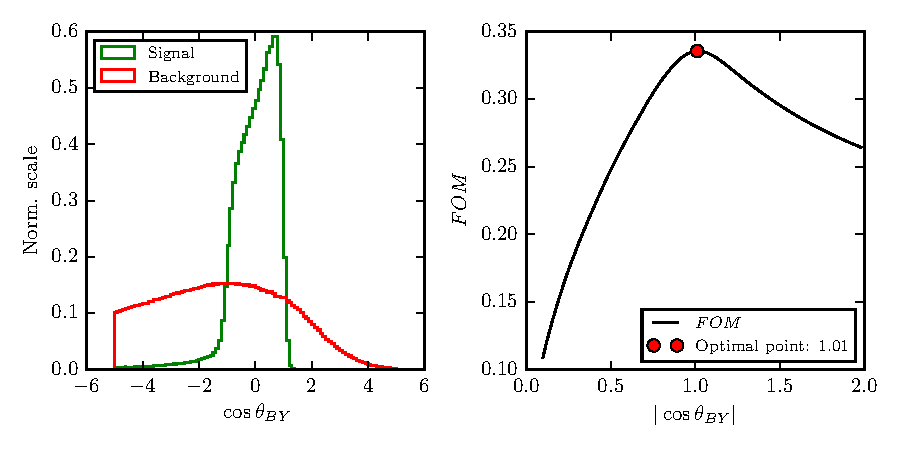
\includegraphics[width=\linewidth]{fig/cosBY}
	\caption{Normalized $\cos \theta_{BY}$ distribution for signal and background $B$ meson candidates (left) and $\mathrm{FOM}$ optimization of the $\cos \theta_{BY}$ variable (right) for the subset of the full Belle MC.}
	\label{fig:cosby}
\end{figure}

We again impose an under-optimized cut on this variable from Figure \ref{fig:cosby} (right) to discard a large amount of background on this subset of the full Belle MC
\begin{itemize}
	\item $\vert \cos \left(\theta_{BY}\right) \vert < 1.20$.
\end{itemize}

\section{Loose Neutrino Reconstruction}\label{sec:loose-neutrino-reconstruction}

%Due to the beam background in the detector, material interactions, or other processes, random tracks and clusters enter our event and get reconstructed as part of the physics process we want to study. These tracks and clusters are not interesting and further spoil the data we measure. In order to remedy this, we perform an extensive clean-up of the tracks and clusters in the ROE side before calculating the four-momentum of the missing part of the event. The clean-up procedure is performed separately on tracks and clusters and uses multiple steps with multivariate analysis (MVA) algorithms in order to separate good tracks and clusters from the bad ones, which populate the ROE. Then, for each ROE object, a ROE mask is created for tracks and clusters, which narrates the use of this track or cluster in the final calculations of the ROE four-momentum.
%
%In order to preserve the continuity of this chapter, a more detailed description of the ROE clean-up can be found in Chapter \ref{ch:roe}. From this point on we assume the ROE to be efficiently cleansed of extra tracks and clusters.


The signal-side neutrino escapes detection, so we cannot directly determine it's four-momentum. However, due to the detectors geometry, which almost completely covers the full solid angle, and due to well known initial conditions of the $\Upsilon(4S)$ meson, it is possible to determine the kinematics of the missing neutrino via indirectly reconstructing the companion $B$ meson by summing up the four-momenta of all the FSP particles in the event which were not used in the reconstruction of the signal side $B$ meson. This is known as the \textit{untagged} method since we are not using any kind of tagging method to reconstruct the companion $B$ meson. The particles used in the indirect companion $B$ meson reconstruction are also said to belong to the \textit{rest of the event} (ROE).

Due to the beam background in the detector, material interactions, or other processes, random tracks and clusters enter our event and get reconstructed as part of the physics process we want to study. These tracks and clusters are not interesting and further spoil the data we measure. In order to remedy this, we perform an extensive clean-up of the tracks and clusters in the ROE side before calculating the four-momentum of the missing part of the event. Here we see the motivation for the ROE clean-up since our signal candidate reconstruction depends on tracks and clusters in the ROE side. The clean-up procedure is performed separately on tracks and clusters and uses multiple steps with multivariate analysis (MVA) algorithms in order to separate good tracks and clusters from the bad ones, which populate the ROE. Then, for each ROE object, a ROE mask is created for tracks and clusters, which narrates the use of this object in the final calculations of the ROE four-momentum. From this point on we assume the ROE to be efficiently cleansed of extra tracks and clusters. A more detailed description of the ROE clean-up can be found in Chapter \ref{ch:roe}. 

The total missing four-momentum in the event can be determined as
\begin{align}
\mathrm{p}_{miss} &= \mathrm{p}_{\Upsilon(4S)} - \sum_i^{\mathrm{Event}}\left(E_i,\,\vec{p}_i \right),\\
\label{eq:ROEloop}
\mathrm{p}_{miss} &= \mathrm{p}_{\Upsilon(4S)} - \left(\mathrm{p}_{Y} -\sum_i^{\mathrm{Rest~of~event}}\left(E_i,\,\vec{p}_i \right)\right),
\end{align}

where the summation runs over all charged and neutral particles in the defined set with
\begin{equation}
\mathrm{p}^{\mathrm{neutral}}_i = \left(p_i,\, \vec{p}_i \right) \quad \mathrm{and} \quad \mathrm{p}^{\mathrm{charged}}_i = \left(\sqrt{m_i^2 + p_i^2},\, \vec{p}_i \right),
\label{eq:pcharged}
\end{equation}
where we assumed all neutral particles to be massless photons. For charged tracks in the ROE a mass hypothesis needs to be defined in order to determine the track's energy. After the ROE clean-up we make the following procedure of choosing the mass hypothesis
\begin{enumerate}
	\item $e$, if $e$ prob. $> \mu$ prob. and $e$ prob. $> 0.9$,
	\item otherwise $\mu$, if $\mu$ prob. $> e$ prob. and $\mu$ prob. $> 0.97$,
	\item otherwise $K$, if $K/\pi$ prob. $> 0.6$,
	\item otherwise $\pi$.
\end{enumerate} 
We define the square of the missing mass, $m_{miss}^2$, which is consistent with zero, if signal-side neutrino is the only missing particle in the event, as shown in Eq. (\ref{eq:m2def}).
\begin{align}
\label{eq:nuold}
\mathrm{p}_\nu &= \mathrm{p}_{miss} = \left(E_{miss},\,\vec{p}_{miss} \right),\\
\label{eq:m2def}
m_{miss}^2 &= \mathrm{p}_{miss}^2 = \mathrm{p}_{\nu}^2 = m_\nu^2 \approx 0.
\end{align}

Since the detector is not perfect, the distribution of the $m_{miss}^2$ variable has a non-zero width. Additionally, a tail is introduced due to missing particles like neutrinos, other neutral undetected particles such as $K_L^0$, or simply missing tracks due to detection failure. Figure \ref{fig:missm2} shows the distribution of $m_{miss}^2$ as defined with the missing four-momentum in Eq. (\ref{eq:nuold}). Correctly reconstructed candidates, which come from events where the other $B$ meson decayed via a hadronic decay mode, peak at zero. If this is not the case, candidates are shifted to larger values of this variable, even if the event in question is a signal event. For this purpose, we define a subset of all signal candidates, which come from events where the companion $B$ meson decayed hadronically and all of its particles were taken into account correctly. We only allow for missing photons, since they are frequently irradiated due to bremsstrahlung effects and they do not have such a big impact on the 4-momentum of the final candidate. We denote this subset as \textit{perfect} signal.

Due to this fact, we impose a cut on the $m_{miss}^2$ variable in order to partially discard candidates with spoiled properties, even if it was in principle a correct combination of FSP particles on the signal side. The cut was chosen based on the optimization of FOM, where in this case the definition of $S$ were perfectly reconstructed signal candidates. The chosen cut value is 
\begin{itemize}
	\item $\vert m_{miss}^2 \vert < 3.0\e{GeV}/c^2$,
\end{itemize}
which is also under-optimized at this point due to the same reasons as in the cases above.


\begin{figure}[H]
	\centering
	\captionsetup{width=.8\linewidth}
	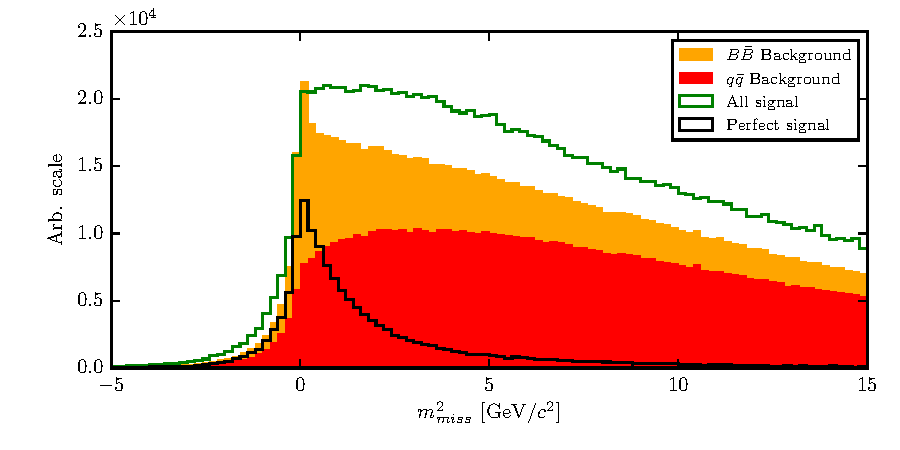
\includegraphics[width=\linewidth]{fig/missM2}
	\caption{Squared missing mass distribution for signal and various types of background. All signal (green) and perfect signal (black) are scaled up equally.}
	\label{fig:missm2}
\end{figure}

The main uncertainty of the neutrino four-momentum, defined in Eq. (\ref{eq:nuold}), comes from energy uncertainty. It is a common practice to substitute the missing energy with the magnitude of the missing momentum, since the momentum resolution from the measurement is much better, thus redefining the neutrino four-momentum to
\begin{equation}
\label{eq:nunew}
\mathrm{p}_\nu = \left(\vert \vec{p}_{miss} \vert,\,\vec{p}_{miss} \right),
\end{equation}
which fixes the neutrino mass to $0\e{GeV}/c^2$.

The newly defined neutrino four-momentum can be added to the four-momentum of the $Y(KK\ell)$ candidate to obtain the full $B$ meson four-momentum and calculate the traditional $M_{BC}$ and $\Delta E$ variables
\begin{align}
\label{eq:de}
\Delta E &= E_B - E_{CMS}/2,\\
M_{BC} &= \sqrt{\left(E_{CMS}/2\right)^2 - \vert \vec{p} \vert^2}.
\end{align}

Since the final fit will be performed over \vars, we define the fit region
\begin{itemize}
	\item $M_{BC} \in [5.1,\,5.295]\e{GeV}/c^2$,
	\item $\Delta E \in [-1.0,\,1.3]\e{GeV}$.
	%\item Signal enhanced region: $M_{BC} \in [5.27,\,5.295]\e{GeV}/c^2$ and $\vert \Delta E \vert < 0.143 \e{GeV}$,
\end{itemize}

Figure \ref{fig:mbc_de_pre} shows the distributions of $\Delta E$ (left) and $M_{BC}$ (right) for signal and major types of background after the pre-cuts. Both signal components are scaled up with respect to the background components but are in proper scale one to another. The effects of missing particles are clearly seen based on the shape difference between all and perfect signal.

\begin{figure}[H]
	\centering
	\captionsetup{width=0.8\linewidth}
	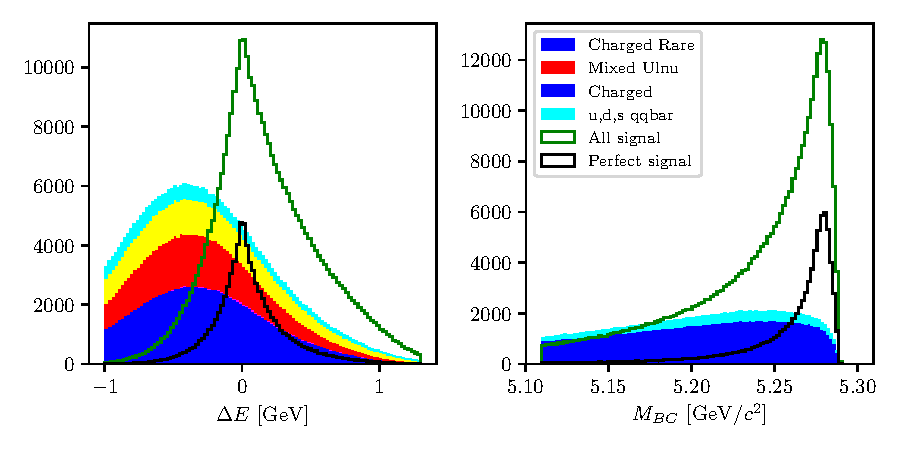
\includegraphics[width=\linewidth]{fig/mbc_de_pre}
	\caption{Distributions of $\Delta E$ (left) and $M_{BC}$ (right) for signal and major types of background after the precuts. Both signal components are scaled up with respect to the background components, but are in proper scale one to another. The perfect signal has a much better resolution in both distributions, since the event is perfectly reconstructed.}
	\label{fig:mbc_de_pre}
\end{figure}

\section{Final Stage Optimization}

With the charge particle selection and a rough selection of the $B$ meson particles in place, we can now afford to run the reconstruction procedure over all $10$ streams of the full available Belle generic MC. After obtaining the full reconstructed sample, the first task is to optimize the under-optimized cuts from the pre-selection stage. Repeating the procedure on the full sample results in the FOM shapes shown in Figure \ref{fig:preciseFOM}, while the optimal cut values are

\begin{itemize}
	\item $P(\chi^2,NDF) > 6.0\E{-3}$,
	\item $\vert \cos \left(\theta_{BY}\right) \vert < 1.05$.
\end{itemize}

\begin{figure}[H]
	\centering
	\captionsetup{width=0.8\linewidth}
	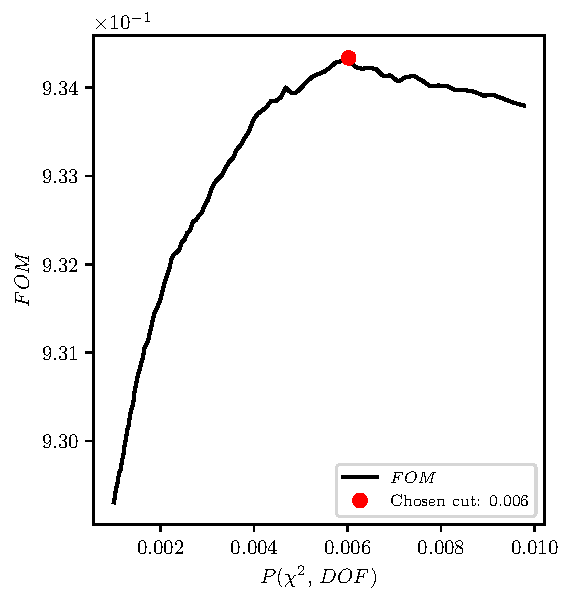
\includegraphics[width=0.48\linewidth]{fig/VTX_precise}
	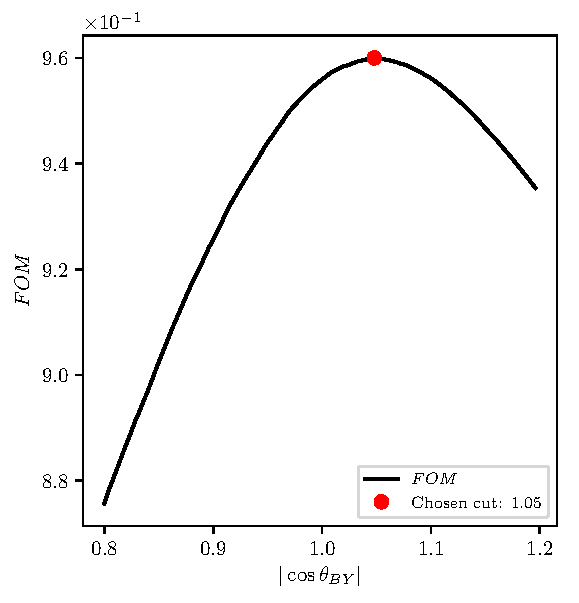
\includegraphics[width=0.48\linewidth]{fig/cosBY_precise}
	\caption{$\mathrm{FOM}$ optimization of the vertex fit probability (left) and the $\cos \theta_{BY}$ variable (right) for the full Belle MC sample.}
	\label{fig:preciseFOM}
\end{figure}

With further optimizations, we will be fine-tuning the signal to background ratio. The most prominent and distinguishable part of our signal is the perfectly reconstructed signal. For this purpose, we define a signal region in \vars, where most of our perfectly reconstructed candidates lie. We use this region for all of the following optimization steps in this chapter and also in the background suppression chapter \ref{sec:background-suppression} since this allows us to better improve the signal to background ratio where it counts most. The 2D $\mathrm{FOM}$ optimization of the optimal \vars~signal region is shown in Figure \ref{fig:sigwin}.

The signal region is defined as
\begin{itemize}
	\item $M_{BC} > 5.271\e{GeV}/c^2.$,
	\item $\vert \Delta E \vert < 0.126\e{Gev}$. 
\end{itemize}

\begin{figure}[H]
	\centering
	\captionsetup{width=0.8\linewidth}
	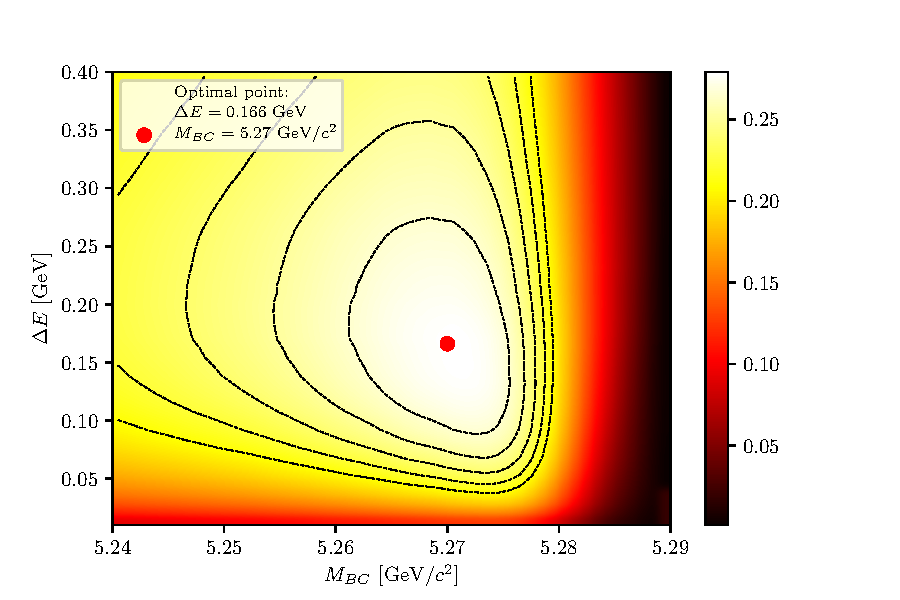
\includegraphics[width=\linewidth]{fig/sigWin}
	\caption{2D $\mathrm{FOM}$ optimization of the signal region definition, where the signal in the optimization was represented by perfectly reconstructed candidates.}
	\label{fig:sigwin}
\end{figure}

With the signal window defined, we can tighten the cut on $m_{miss}^2$, which we intentionally left loose before the signal categorization. With the $\mathrm{FOM}$ optimization of perfectly reconstructed candidates inside the signal region, shown in Figure \ref{fig:missm2opt}, the optimal cut on $m_{miss}^2$ is 

\begin{itemize}
	\item $\vert m_{miss}^2 \vert < 0.975\e{GeV}/c^2$.
\end{itemize}

\begin{figure}[H]
	\centering
	\captionsetup{width=0.8\linewidth}
	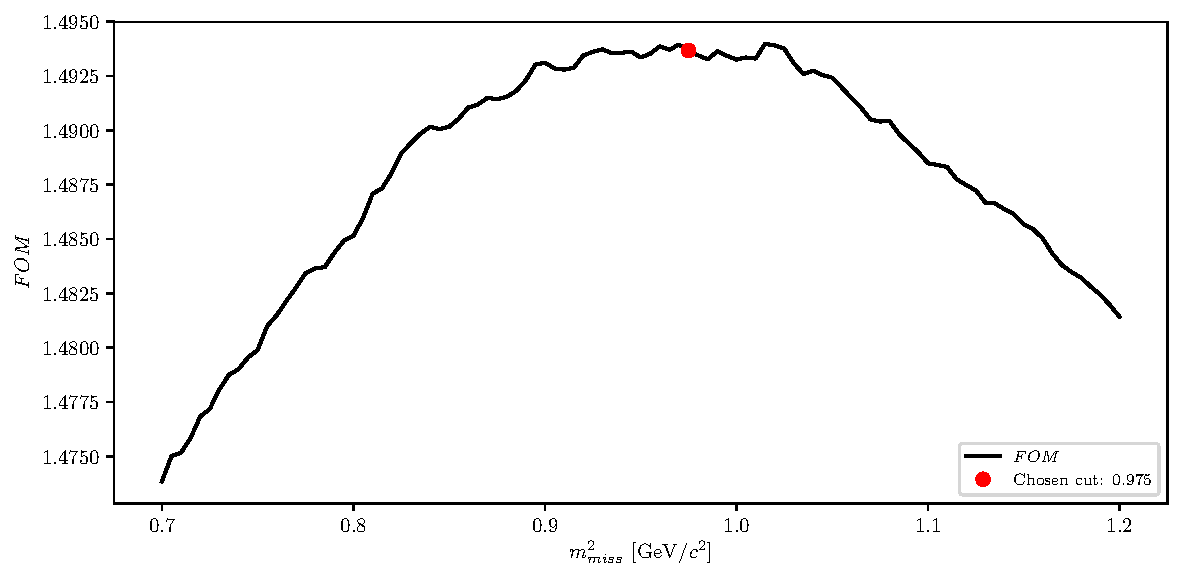
\includegraphics[width=\linewidth]{fig/missM2_precise}
	\caption{$\mathrm{FOM}$ optimization of the optimal $m_{miss}^2$ cut in the signal region.}
	\label{fig:missm2opt}
\end{figure}

\section{Charge product categorization}\label{sec:event-categorization}

The missing information due to an escaping neutrino in our reconstructed channel is replaced by information from the companion $B$ meson. Since this is an untagged reconstruction, the quality of the companion $B$ meson affects the properties of the signal candidate. Perfect reconstruction of a hadronically decayed companion $B$ meson results in pronounced peaks at $\Delta E \approx 0$, $m_{miss}^2 \approx 0$ and $M_{BC} \approx m_B$, while imperfect reconstruction due to any kind of missing particles produces tails, shift or simply a worse resolution of the mentioned distributions. These effects are undesired since they make it harder to separate signal from background.

To remedy this, we look at the charge product of the reconstructed $B$ meson and the ROE object. For correctly reconstructed events, this should have a value of 
\begin{equation}
\label{eq:chargeprod}
q_{B^\pm}q_{B^\mp} = -1,
\end{equation}

however, this value is distributed due to missing charged particles in the reconstruction. Figure \ref{fig:sig_categ} shows various signal distributions of \vars~in arbitrary (left) and normalized (right) scales, with the relative ratios of $67.86~\%$ and $32.14~\%$ for correct and wrong values of the charge product, respectively. We see that correctly reconstructed events represent the majority of signal and also have the best resolution in \vars, so we proceed with the analysis by imposing the cut in Eq. \ref{eq:chargeprod}.

While this cut introduces a drop in the signal efficiency of about $32.14~\%$, it improves the resolution of our signal \vars~distributions and also the signal to background ratio, where the latter changes from $0.95\E{-3}$ to $1.09\E{-3}$.

\begin{figure}[H]
	\centering
	\captionsetup{width=0.8\linewidth}
	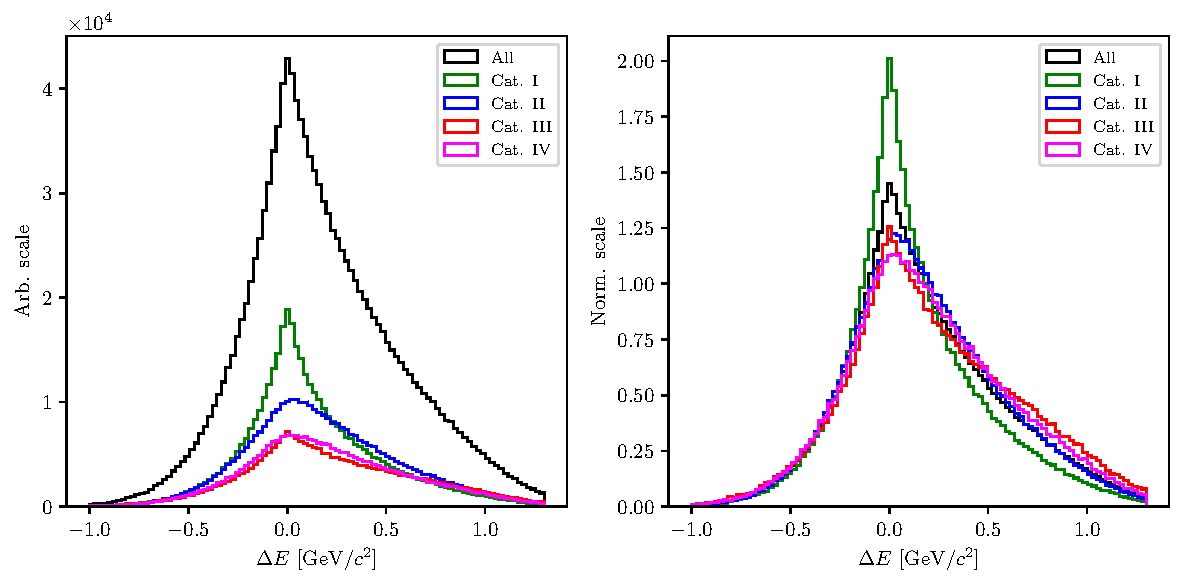
\includegraphics[width=\linewidth]{fig/sig_categ}
	\caption{Signal distributions of \vars~based on the charge product of both $B$ mesons in the event. The plot on the left shows the distributions in an arbitrary scales, while the plot on the right shows the normalized distributions.}
	\label{fig:sig_categ}
\end{figure}

\section{Selection Summary}
\label{s:ss}
In this section, one can find the full summary of all final selection cuts in the event reconstruction, from FSP particles up to the $B$ meson.

\begin{itemize}
	\item FSP particles:
	\begin{itemize}
		\item electrons: $\vert d_0 \vert < 0.1\e{cm},\,\vert z_0 \vert < 1,5\e{cm},\,p>0.6\e{GeV}/c,\\p_{CMS}\in[0.4,\,2.6]\e{GeV}/c,\,eID>0.9,$
		\item muons: $\vert d_0 \vert < 0.1\e{cm},\,\vert z_0 \vert < 1,5\e{cm},\,p_{CMS}\in[0.6,\,2.6]\e{GeV}/c,\\\mu ID>0.97,$
		\item kaons: $\vert d_0 \vert < 0.15\e{cm},\,\vert z_0 \vert < 1,5\e{cm},\,p_{CMS} < 2.5\e{GeV}/c,\\K/\pi~ID>0.6,\,K/p~ID>0.1,$
	\end{itemize}
	\item $B$ meson candidates:
	\begin{itemize}
		\item standard cuts: $P(\chi^2,\,DOF) > 6\E{-3},\,\vert \cos \theta_{BY} \vert < 1.05,\,\vert m_{miss}^2\vert<0.975\e{GeV}/c^2,$
		\item fit region cuts: $\Delta E \in [-1.0,1.3]\e{GeV},\,M_{BC} \in [5.1,5.295]\e{GeV}/c^2,$
		\item signal region cuts: $\vert \Delta E \vert < 0.126\e{GeV},\,M_{BC} > 5.271\e{GeV}/c^2,$
		\item charge categorization: $q_{B^\pm}q_{B^\mp} = -1.$
	\end{itemize}
\end{itemize}